\documentclass[aspectratio=169,10pt]{beamer}
\usetheme{default}
\usepackage{amsmath,amssymb,booktabs,graphicx,tikz,listings}
\usetikzlibrary{arrows.meta,positioning}
\definecolor{navy}{HTML}{14243A}\definecolor{blue}{HTML}{2878B5}\definecolor{teal}{HTML}{159A8C}\definecolor{coral}{HTML}{E76F51}\definecolor{ink}{HTML}{233247}\definecolor{muted}{HTML}{607086}\definecolor{paper}{HTML}{F6F8FB}\definecolor{paleBlue}{HTML}{EAF2F9}\definecolor{paleTeal}{HTML}{E8F5F2}
\setbeamercolor{normal text}{fg=ink,bg=paper}\setbeamercolor{frametitle}{fg=navy,bg=white}\setbeamercolor{structure}{fg=teal}\setbeamercolor{block title}{fg=white,bg=navy}\setbeamercolor{block body}{fg=ink,bg=white}\setbeamercolor{alerted text}{fg=coral}
\setbeamertemplate{navigation symbols}{}\setbeamertemplate{itemize item}{\color{teal}\scriptsize$\blacktriangleright$}
\setbeamertemplate{frametitle}{\nointerlineskip\begin{beamercolorbox}[wd=\paperwidth,ht=3.2ex,dp=1.1ex,leftskip=.55cm,rightskip=.55cm]{frametitle}\usebeamerfont{frametitle}\insertframetitle\end{beamercolorbox}\vspace{-.1em}\hspace{.55cm}{\color{teal}\rule{1.2cm}{1.2pt}}\hspace{.15cm}{\color{blue}\rule{.45cm}{1.2pt}}\par\vspace{.25em}}
\setbeamertemplate{footline}{\leavevmode\hbox{\begin{beamercolorbox}[wd=.82\paperwidth,ht=2.5ex,dp=1ex,leftskip=.55cm]{author in head/foot}\color{muted}\scriptsize ADAM  /  ANALYSIS OF ALGORITHMS  /  PRESENTATION I\end{beamercolorbox}\begin{beamercolorbox}[wd=.18\paperwidth,ht=2.5ex,dp=1ex,rightskip=.55cm plus1fil]{date in head/foot}\color{navy}\scriptsize\insertframenumber\,/\,10\end{beamercolorbox}}}
\setbeamersize{text margin left=.58cm,text margin right=.58cm}
\lstset{language=C++,basicstyle=\ttfamily\scriptsize,keywordstyle=\color{blue}\bfseries,commentstyle=\color{muted},numbers=left,numberstyle=\tiny\color{muted},numbersep=5pt,showstringspaces=false,breaklines=true,tabsize=2,aboveskip=.2em,belowskip=.2em}
\newcommand{\timing}[1]{\hfill{\color{teal}\scriptsize\bfseries #1}}
\newcommand{\metric}[3]{\begin{beamercolorbox}[rounded=true,sep=.45em,center,wd=\linewidth]{block body}\textcolor{#1}{\Large\bfseries #2}\\[-.2ex]{\scriptsize #3}\end{beamercolorbox}}
\title{Adam: From Adaptive Updates to Experimental Evidence}\author{Dario Pomasqui}\institute{Yachay Tech University \;|\; Analysis of Algorithms}\date{Presentation I}
\begin{document}

% 0:25 ? Introduce the topic and central question.
\begin{frame}[plain]
\setbeamercolor{background canvas}{bg=navy}
\begin{tikzpicture}[remember picture,overlay]\fill[navy](current page.south west)rectangle(current page.north east);\fill[teal,opacity=.14]([xshift=-.1cm]current page.east)circle[radius=5.3cm];\fill[blue,opacity=.12]([xshift=-1.4cm,yshift=-1.2cm]current page.east)circle[radius=3.6cm];\end{tikzpicture}
\vspace{.55cm}\begin{columns}[T,onlytextwidth]
\begin{column}{.58\textwidth}{\color{teal}\bfseries\small ANALYSIS OF ALGORITHMS  /  PRESENTATION I}\par\vspace{.65cm}{\color{white}\fontsize{28}{32}\selectfont\bfseries Adam}\par{\color{white}\fontsize{18}{22}\selectfont Adaptive Moment Estimation}\par\vspace{.7cm}{\color{white}\large How does Adam behave across objective landscapes, and what changes when we compare it with Momentum and AMSGrad?}\par\vspace{.75cm}{\color{white!72}\normalsize Dario Pomasqui\\Yachay Tech University}\end{column}
\begin{column}{.37\textwidth}\centering\begin{tikzpicture}[scale=.93]\draw[white,opacity=.22,line width=1pt,rotate around={-28:(0,0)}](0,0)ellipse(.55 and .30);\draw[white,opacity=.22,line width=1pt,rotate around={-28:(0,0)}](0,0)ellipse(1.05 and .58);\draw[white,opacity=.22,line width=1pt,rotate around={-28:(0,0)}](0,0)ellipse(1.55 and .85);\draw[white,opacity=.22,line width=1pt,rotate around={-28:(0,0)}](0,0)ellipse(2.05 and 1.13);\draw[teal,line width=2.5pt,-{Stealth[length=3mm]}](2.35,1.15)..controls(1.75,.95)and(1.45,.12)..(.72,.25)..controls(.35,.31)and(.32,-.12)..(0,0);\fill[coral](2.35,1.15)circle(2.4pt);\fill[teal](0,0)circle(3.4pt);\node[white,anchor=west,font=\scriptsize]at(2.32,1.35){start};\node[white,anchor=north east,font=\scriptsize]at(-.08,-.08){minimum};\end{tikzpicture}
\vspace{.28cm}\begin{beamercolorbox}[rounded=true,sep=.55em,wd=\linewidth,left]{block body}
{\color{muted}\scriptsize\bfseries PROJECT RESOURCES}\par\vspace{.18em}
\href{https://www.overleaf.com/project/6adbd768cbee7aeb66bcd5f9/share\#1b64dd9bd84fd0003f81626d5a4e47af269068164341fd83}{\textcolor{blue}{\small\bfseries 1. OVERLEAF MANUSCRIPT}}\par\vspace{.14em}
\href{https://github.com/darioXxx32/Algorithm-analysis/tree/main/Adam-Analysis}{\textcolor{blue}{\small\bfseries 2. GITHUB REPOSITORY}}\par\vspace{.14em}
\href{https://drive.google.com/drive/folders/1WUl1pRtYdUr3mXK9QRBEN3LEOtXKuQGO?usp=drive_link}{\textcolor{blue}{\small\bfseries 3. PRESENTATION VIDEO}}
\end{beamercolorbox}\end{column}
\end{columns}\end{frame}

% 0:50 - Explain importance and scope.
\begin{frame}{Why adaptive optimization? \timing{0:50}}
\begin{center}{\large Optimization repeatedly adjusts parameters to reduce an objective.}\end{center}\vspace{.2cm}
\begin{columns}[T,onlytextwidth]
\begin{column}{.32\textwidth}\begin{block}{Problem addressed}\small A single global step size can be awkward when coordinates have different gradient scales or the objective has uneven geometry.\end{block}\end{column}
\begin{column}{.32\textwidth}\begin{block}{Adam's idea}\small Smooth recent gradients for a direction; use recent squared gradients to scale each coordinate's step.\end{block}\end{column}
\begin{column}{.32\textwidth}\begin{block}{Why study it?}\small Adaptive optimizers are widely used in machine learning. Understanding their updates and limits matters beyond calling a library.\end{block}\end{column}
\end{columns}\vspace{.25cm}
\begin{beamercolorbox}[rounded=true,sep=.65em,wd=\textwidth]{block body}\textbf{Research question:} On deterministic test functions, how do Adam's convergence observations and cost compare with SGD+Momentum and AMSGrad?\\[.25em]\textcolor{muted}{Scope: analytic objectives and a prescribed gradient sequence; not a neural-network training benchmark.}\end{beamercolorbox}
\note{Adam is practically relevant, while our evidence comes from small deterministic experiments, not neural network training.}\end{frame}

% 1:20 - Explain the vector recurrence and visual data flow.
\begin{frame}{One Adam step: direction, scale, correction \timing{1:20}}
\begin{columns}[T,onlytextwidth]\begin{column}{.54\textwidth}\vspace{.1cm}\small
\[g_t=\nabla f(\theta_t),\quad m_t=\beta_1m_{t-1}+(1-\beta_1)g_t\]
\[v_t=\beta_2v_{t-1}+(1-\beta_2)g_t\odot g_t\]
\[\widehat m_t=\frac{m_t}{1-\beta_1^t},\quad\widehat v_t=\frac{v_t}{1-\beta_2^t}\]
\[\theta_{t+1}=\theta_t-\alpha\frac{\widehat m_t}{\sqrt{\widehat v_t}+\epsilon}\]
\begin{beamercolorbox}[rounded=true,sep=.5em,wd=\linewidth]{block body}\scriptsize State starts at $m_0=v_0=0$; increment $t$ before correction. Square, square root and division are element-wise. $\epsilon$ is \textbf{outside} the square root.\end{beamercolorbox}
\end{column}\begin{column}{.44\textwidth}\centering
\resizebox{\linewidth}{!}{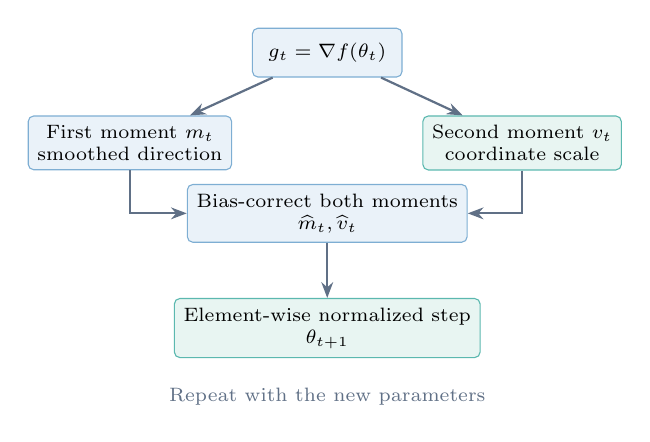
\begin{tikzpicture}[node distance=.48cm and .25cm,every node/.style={font=\scriptsize,align=center},box/.style={rounded corners=2pt,draw=blue!60,fill=paleBlue,minimum width=1.9cm,minimum height=.62cm},tealbox/.style={rounded corners=2pt,draw=teal!70,fill=paleTeal,minimum width=1.9cm,minimum height=.62cm},arr/.style={-{Stealth[length=2mm]},thick,draw=muted}]
\node[box](grad){$g_t=\nabla f(\theta_t)$};\node[box,below left=of grad](m){First moment $m_t$\\smoothed direction};\node[tealbox,below right=of grad](v){Second moment $v_t$\\coordinate scale};\node[box,below=1.35cm of grad](bias){Bias-correct both moments\\$\widehat m_t,\widehat v_t$};\node[tealbox,below=.70cm of bias](step){Element-wise normalized step\\$\theta_{t+1}$};\draw[arr](grad)--(m);\draw[arr](grad)--(v);\draw[arr](m)|-(bias);\draw[arr](v)|-(bias);\draw[arr](bias)--(step);\node[below=.25cm of step,text=muted]{Repeat with the new parameters};
\end{tikzpicture}}\end{column}\end{columns}
\note{The first moment smooths direction; the second tracks coordinate scale. Bias correction compensates for zero initialization. Point out epsilon placement.}\end{frame}

% 0:45 - Give the complete Adam procedure and classify its paradigm and cost.
\begin{frame}{Adam in pseudocode: the main algorithm \timing{0:45}}
\begin{columns}[T,onlytextwidth]
\begin{column}{.64\textwidth}
\begin{beamercolorbox}[rounded=true,sep=.35em,wd=\linewidth]{block body}
\scriptsize\textbf{Input:} objective $f$, gradient $\nabla f$, initial vector $\theta_0$, rate $\alpha$, $\beta_1,\beta_2,\epsilon$, limit $T$\\
\textbf{Initialize:} $m_0\gets\mathbf0$, $v_0\gets\mathbf0$\\
\textbf{For} $t=1,\ldots,T$:\\
\hspace{1em}$g_t\gets\nabla f(\theta_{t-1})$\\
\hspace{1em}$m_t\gets\beta_1m_{t-1}+(1-\beta_1)g_t$\\
\hspace{1em}$v_t\gets\beta_2v_{t-1}+(1-\beta_2)(g_t\odot g_t)$\\
\hspace{1em}$\widehat m_t\gets m_t/(1-\beta_1^t)$; $\widehat v_t\gets v_t/(1-\beta_2^t)$\\
\hspace{1em}$\theta_t\gets\theta_{t-1}-\alpha\widehat m_t/(\sqrt{\widehat v_t}+\epsilon)$\\
\hspace{1em}\textbf{Stop if} configured criterion is met\\
\textbf{Return:} $\theta_t$
\end{beamercolorbox}
\end{column}
\begin{column}{.33\textwidth}
\begin{block}{Algorithmic paradigm}\small Iterative, first-order, gradient-based optimization. Adam adapts each coordinate using exponential moving averages of gradient moments. It supports stochastic gradients; these experiments use deterministic objectives.\end{block}
\begin{beamercolorbox}[rounded=true,sep=.55em,wd=\linewidth]{block body}\textbf{Adam complexity}\\[.25em]\small Update time: $O(d)$ per step, given the gradient.\\[.25em]Optimizer state: $m_t,v_t$, so $O(d)$ auxiliary memory.\end{beamercolorbox}
\end{column}
\end{columns}
\vspace{.05cm}\centering\tiny $d$ is the number of parameters. Gradient-computation cost is additional; model and parameter storage are excluded from optimizer auxiliary state.
\note{Adam is the project’s main algorithm. It is iterative first-order gradient optimization with adaptive coordinate-wise scaling, not a divide-and-conquer paradigm. With the gradient supplied, moment and parameter updates scan d coordinates. The stored moment vectors take O(d) auxiliary memory. Momentum and AMSGrad are comparison methods only.}
\end{frame}

% 1:10 - Show how the recurrence maps into the C++ implementation.
\begin{frame}[fragile]{C++17 implementation of Adam \timing{1:10}}
\begin{columns}[T,onlytextwidth]\begin{column}{.58\textwidth}\begin{beamercolorbox}[rounded=true,sep=.4em,wd=\linewidth]{block body}\begin{lstlisting}
if (t == 0) { m.assign(d, 0.0); v.assign(d, 0.0); }
++t;
const double bc1 = 1.0 - std::pow(beta1, t);
const double bc2 = 1.0 - std::pow(beta2, t);
for (size_t i = 0; i < d; ++i) {
    m[i] = beta1*m[i] + (1-beta1)*grads[i];
    v[i] = beta2*v[i] + (1-beta2)*grads[i]*grads[i];
    const double mhat = m[i] / bc1;
    const double vhat = v[i] / bc2;
    const double update = learning_rate * mhat /
        (std::sqrt(vhat) + epsilon);
    params[i] -= update;
}
\end{lstlisting}
\end{beamercolorbox}\end{column}
\begin{column}{.39\textwidth}\begin{block}{Project design}\small \texttt{Optimizer::step} accepts parameter and gradient vectors.\\[.3em]Objective functions return $f(\theta)$ and fill a gradient vector.\\[.3em]\texttt{reset()} clears state between runs.\\[.3em]\textbf{Adam settings:} $\beta_1=.9$, $\beta_2=.999$, $\epsilon=10^{-8}$; $\alpha$ varies by objective.\end{block}\begin{beamercolorbox}[rounded=true,sep=.5em,wd=\linewidth]{block body}\textbf{Safety checks}\\[-.1em]\scriptsize Finite positive learning rate; valid $\beta$ and $\epsilon$; matching dimensions; finite inputs and updates. Invalid cases throw exceptions.\end{beamercolorbox}\vspace{.25em}\scriptsize Tests check known gradients, first updates, reset, invalid hyperparameters, dimension changes and non-finite gradients.\end{column}\end{columns}
\note{The vectors store moments; scalar bias factors are computed once, then each coordinate updates in place. The implementation is directly in C++, not a PyTorch wrapper.}
\end{frame}

% 1:00 - Establish design, metrics and validation; Adam is the main algorithm.
\begin{frame}{Experiments: Adam and comparison methods \timing{1:00}}
\begin{columns}[T,onlytextwidth]\begin{column}{.63\textwidth}\small
\begin{tabular}{@{}p{1.6cm}p{2.9cm}p{2.25cm}@{}}\toprule
\textbf{Test}&\textbf{Start $\rightarrow$ target}&\textbf{Stop rule}\\\midrule
Quad 2D&$(5,-3)\rightarrow(0,0)$&$\|g\|_2<10^{-8}$\\
Quad 10D&10D vector $\rightarrow\mathbf0$&$\|g\|_2<10^{-8}$\\
Rosenbrock&$(-1.5,2)\rightarrow(1,1)$&$\|g\|_2<10^{-6}$\\
Rastrigin 2D&$(2.5,2.5)\rightarrow(0,0)$&$\|g\|_2<10^{-6}$\\
Reddi&$x_0=0\rightarrow$ target $-1$&300k fixed steps\\\bottomrule\end{tabular}
\end{column}\begin{column}{.34\textwidth}\begin{block}{Study design}\scriptsize Main algorithm: \textbf{Adam}.\\Comparisons: SGD+Momentum, $u_t=\beta u_{t-1}+g_t$; AMSGrad, $v_t^{\max}=\max(v_{t-1}^{\max},v_t)$.\end{block}\begin{beamercolorbox}[rounded=true,sep=.5em,wd=\linewidth]{block body}\textbf{Fairness choices}\\[-.1em]\scriptsize Same start, cap and stopping rule. Rates (Adam/Momentum/AMSGrad): quadratic $.01/.01/.01$; Rosenbrock $.01/.001/.01$; Rastrigin $.05/.005/.05$. No equal tuning budget.\end{beamercolorbox}\end{column}\end{columns}
\vspace{.2cm}\centering\scriptsize C++17 / CMake runner \quad$\bullet$\quad CSV: loss, gradient norm, distance, coordinates \quad$\bullet$\quad plots from CSV \quad$\bullet$\quad CTest: 1/1 passed
\note{The first four tests use analytic gradients and known minimizers. Reddi supplies a periodic gradient, projects x onto [-1,1], and runs for a fixed budget.}\end{frame}

% 1:20 - Report actual Rosenbrock curves and iteration counts.
\begin{frame}{Rosenbrock: Adam and comparison results \timing{1:20}}
\begin{center}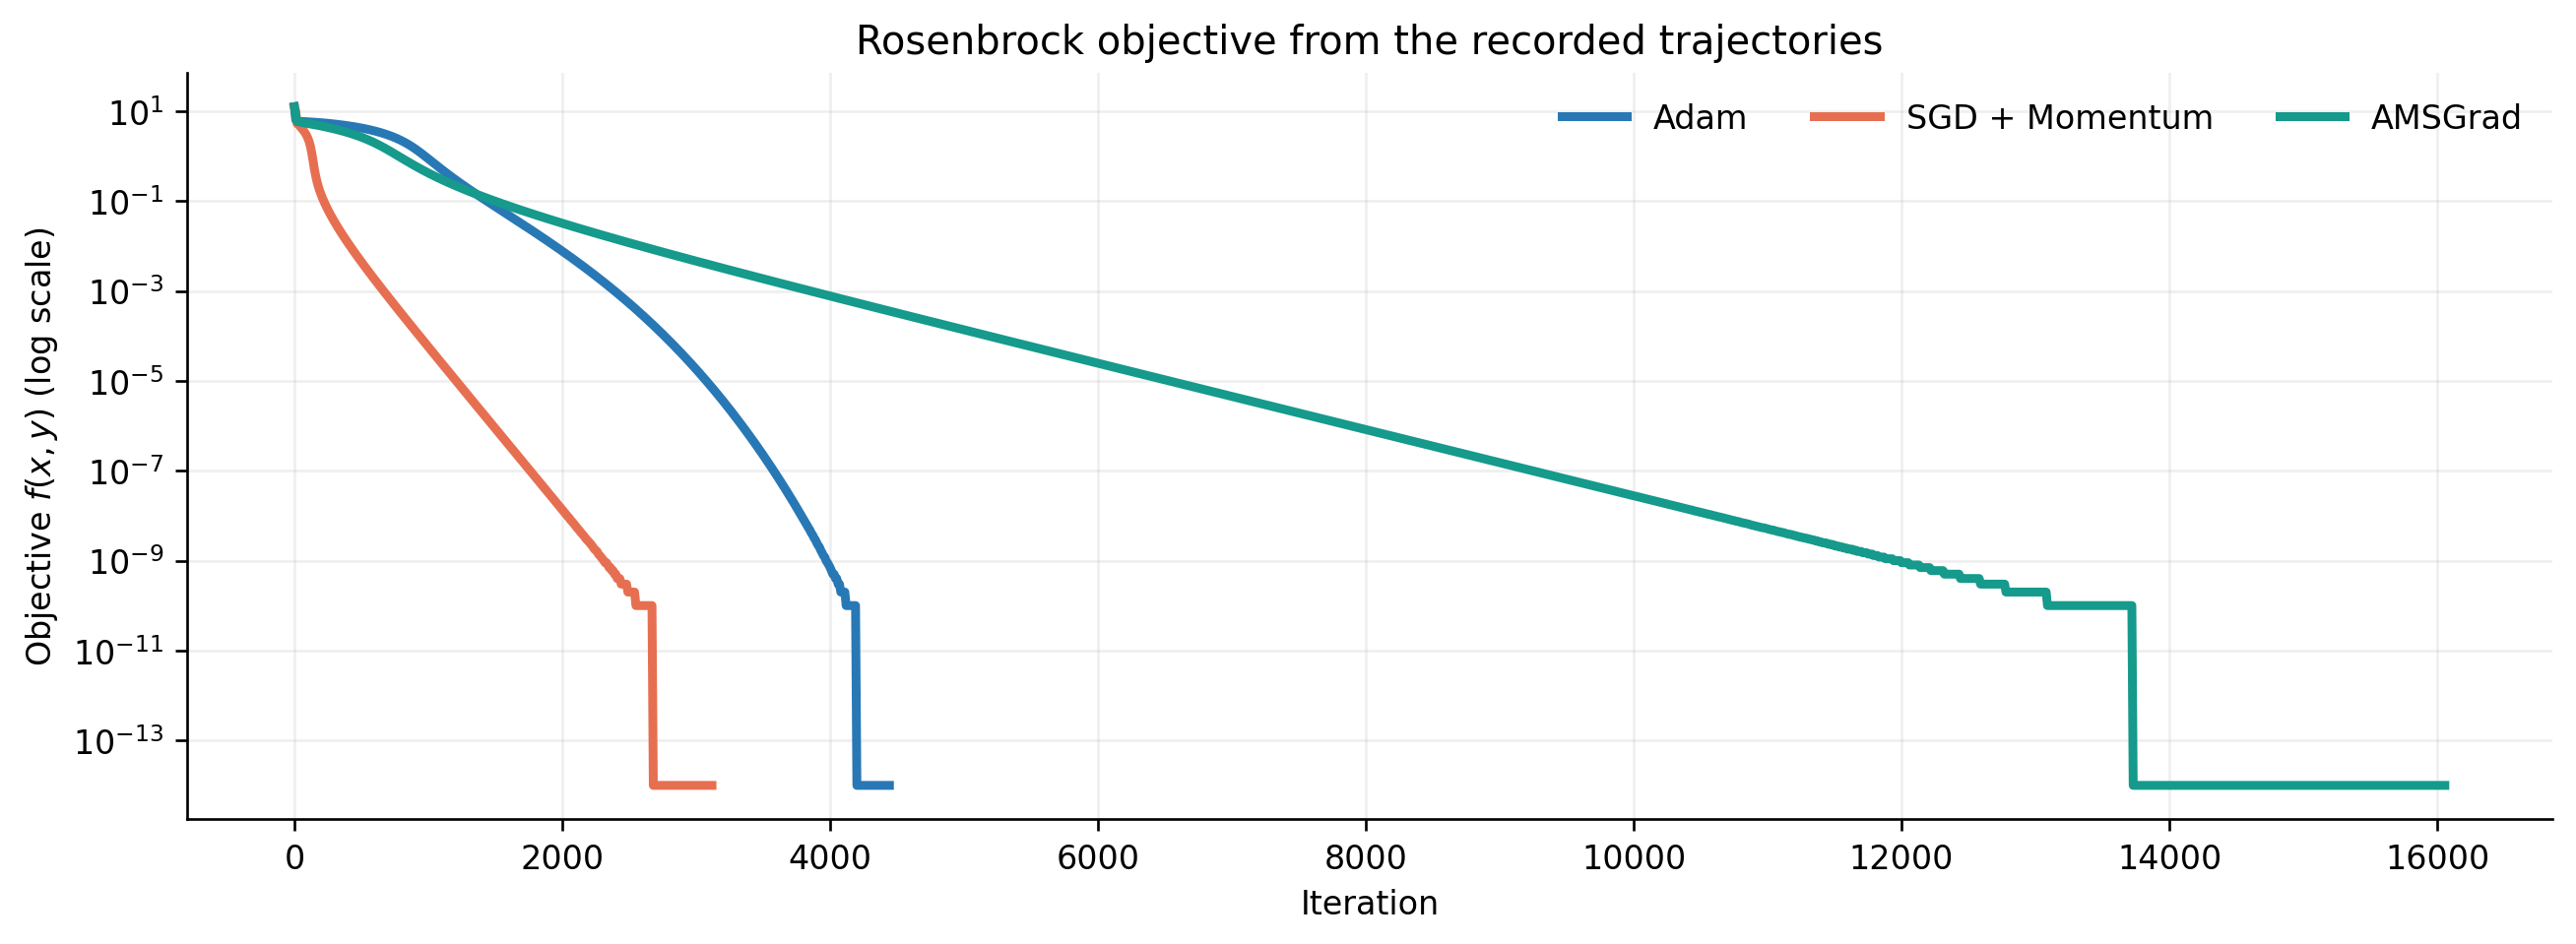
\includegraphics[width=.96\textwidth,height=.56\textheight,keepaspectratio]{presentation_assets/rosenbrock_loss.png}\end{center}\vspace{-.05cm}
\begin{columns}[c,onlytextwidth]\begin{column}{.31\textwidth}\metric{blue}{4,443}{Adam updates to $\|\nabla f\|<10^{-6}$}\end{column}\begin{column}{.31\textwidth}\metric{coral}{3,118}{SGD + Momentum updates}\end{column}\begin{column}{.31\textwidth}\metric{teal}{16,057}{AMSGrad updates}\end{column}\end{columns}
\note{All three reach the configured threshold. Momentum needs the fewest updates here, AMSGrad the most; this is not a universal ranking.}\end{frame}

% 1:15 - Explain non-global stationary points and the finite Reddi illustration.
\begin{frame}{Adam on multimodal and prescribed gradients \timing{1:15}}
\begin{columns}[T,onlytextwidth]\begin{column}{.37\textwidth}\textbf{Rastrigin, start $(2.5,2.5)$}\par\vspace{.1cm}\scriptsize All runs satisfy $\|\nabla f\|<10^{-6}$, but the known global objective is $0$.\par\vspace{.15cm}
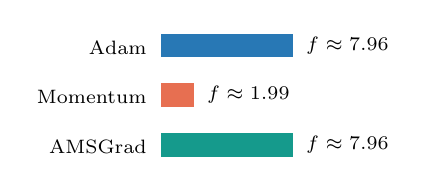
\begin{tikzpicture}[x=.40cm,y=.63cm]\node[anchor=east,font=\scriptsize]at(1.7,2.2){Adam};\node[anchor=east,font=\scriptsize]at(1.7,1.2){Momentum};\node[anchor=east,font=\scriptsize]at(1.7,.2){AMSGrad};\fill[blue](1.85,2)rectangle(6.05,2.48);\fill[coral](1.85,1)rectangle(2.90,1.48);\fill[teal](1.85,0)rectangle(6.05,.48);\node[anchor=west,font=\scriptsize]at(6.15,2.24){$f\approx7.96$};\node[anchor=west,font=\scriptsize]at(3.00,1.24){$f\approx1.99$};\node[anchor=west,font=\scriptsize]at(6.15,.24){$f\approx7.96$};\end{tikzpicture}\par\vspace{.12cm}\begin{beamercolorbox}[rounded=true,sep=.45em,wd=\linewidth]{block body}\scriptsize One start illustrates local minima; it does not estimate global success rates.\end{beamercolorbox}
\end{column}\begin{column}{.57\textwidth}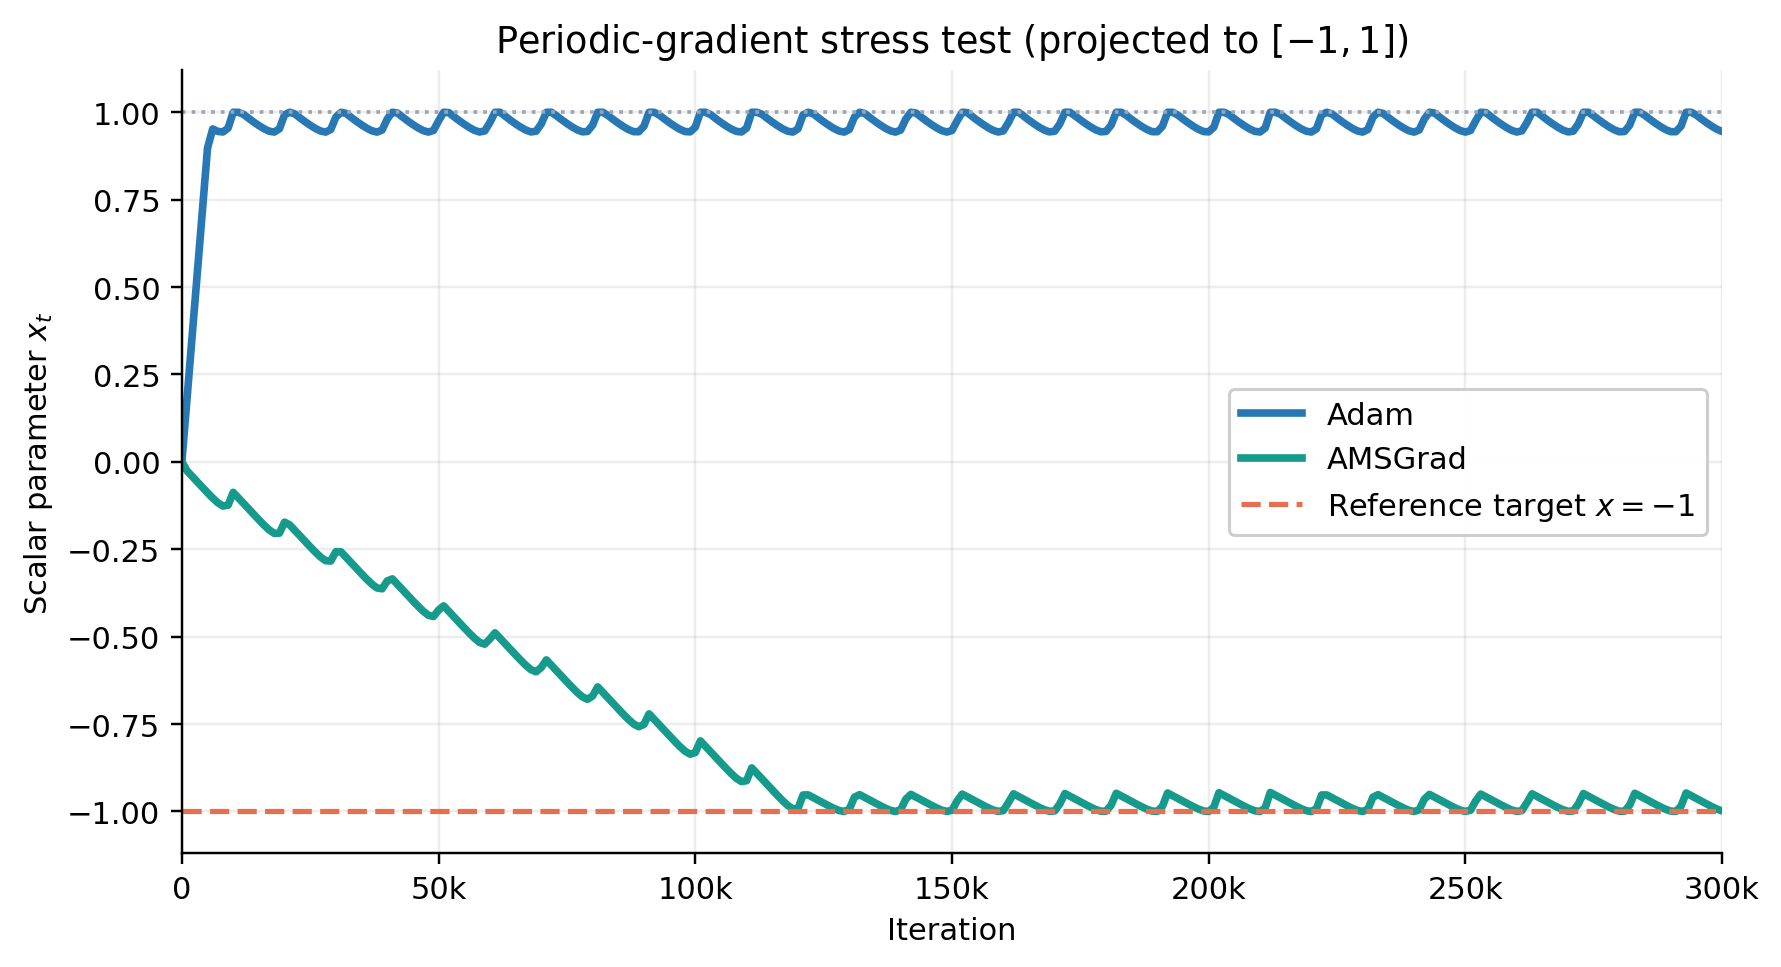
\includegraphics[width=\linewidth,height=.50\textheight,keepaspectratio]{presentation_assets/reddi_trajectory.png}\par\vspace{.05cm}\parbox{\linewidth}{\scriptsize Finite projected schedule from $x_0=0$; $\alpha=.01$, $\beta_1=.9$, $\beta_2=.99$. Endpoints: Adam $0.9454$, AMSGrad $-0.9982$ (target $-1$).}\end{column}\end{columns}
\note{Rastrigin meets a gradient threshold at non-global stationary points. The Reddi plot is one finite prescribed schedule; it illustrates distinct outcomes, not a universal theorem.}\end{frame}

% 1:00 - Address Adam learning-rate sensitivity.
\begin{frame}{Adam learning-rate sensitivity \timing{1:00}}
\begin{columns}[T,onlytextwidth]\begin{column}{.64\textwidth}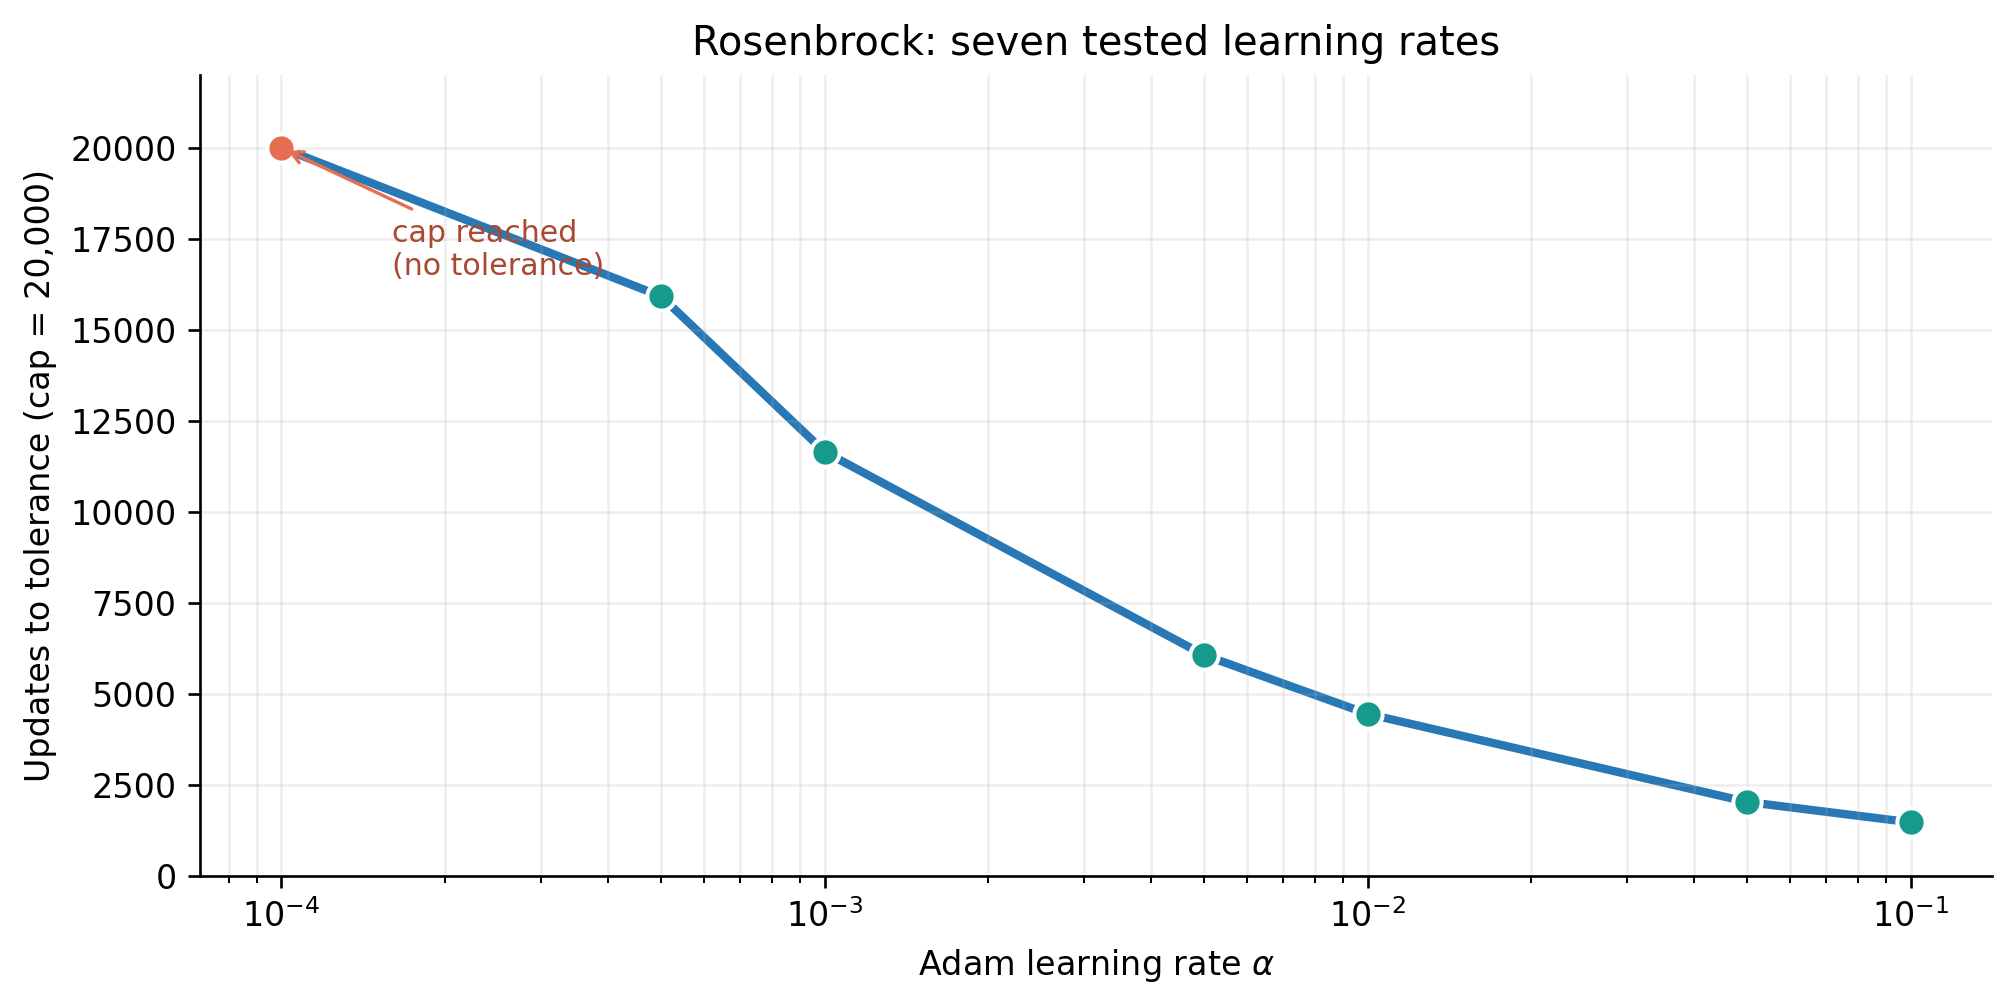
\includegraphics[width=\linewidth,height=.50\textheight,keepaspectratio]{presentation_assets/learning_rate_sweep.png}\par\vspace{.1cm}\parbox{\linewidth}{\scriptsize Adam on Rosenbrock; one fixed start. The lowest tested rate reaches the cap without meeting tolerance.}\end{column}\begin{column}{.31\textwidth}\begin{block}{Interpretation}\small The learning rate changes Adam's observed progress on this objective. The smallest tested rate reached the iteration cap. This supports sensitivity in the tested grid only.\end{block}\begin{beamercolorbox}[rounded=true,sep=.5em,wd=\linewidth]{block body}\scriptsize Timing is from one run, not a performance benchmark.\end{beamercolorbox}\end{column}\end{columns}
\note{Within this tested grid, larger rates took fewer steps to tolerance, while 1e-4 reached the cap. Do not extrapolate outside the grid. Complexity excludes gradient computation.}\end{frame}

% 0:55 - Close with supported claims, limitations and references.
\begin{frame}{Adam: conclusions and limits \timing{0:55}}
\begin{columns}[T,onlytextwidth]\begin{column}{.32\textwidth}\begin{block}{Main contribution}\small Adam is implemented in C++17 for parameter vectors, with bias correction and numerical checks.\end{block}\end{column}\begin{column}{.32\textwidth}\begin{block}{Evidence}\small Outcomes change with the objective and rate; a small gradient did not imply the Rastrigin global minimum.\end{block}\end{column}\begin{column}{.32\textwidth}\begin{block}{Comparison role}\small Momentum and AMSGrad are comparison baselines. No method is shown to be universally superior.\end{block}\end{column}\end{columns}\vspace{.1cm}
\begin{beamercolorbox}[rounded=true,sep=.45em,wd=\textwidth]{block body}\scriptsize\textbf{Limits:} small deterministic tests; one start per objective; no equal tuning budget; single-run timing; finite Reddi construction. No universal superiority or convergence claim.\\[.2em]\textbf{References:} D. P. Kingma and J. Ba, ``Adam: A Method for Stochastic Optimization,'' ICLR (2015).\quad S. J. Reddi, S. Kale, and S. Kumar, ``On the Convergence of Adam and Beyond,'' ICLR (2018).\quad B. T. Polyak, ``Some Methods of Speeding up the Convergence of Iteration Methods'' (1964).\end{beamercolorbox}\vspace{.35cm}\centering{\color{navy}\Large Thank you}\par\vspace{.1cm}{\color{muted}\small Questions?}
\note{Close with correct implementation and reproducible observations under declared settings; then name limitations and invite questions.}\end{frame}
\end{document}

